\section{绪论}
\subsection{研究背景与意义}

在计算机视觉领域,图像的预处理技术至关重要,因为它们可以显著提高图像分析任务的效率和准确性。超像素生成技术作为其中一种重要的预处理手段,通过将图像分割成在视觉上相似且形状规则的像素块,有助于减少图像数据的复杂性,从而降低后续处理的计算成本。然而,现有的超像素生成算法在生成具有良好形状规则性和边界贴合度的超像素时面临挑战,尤其是在需要生成较少数量超像素的场景下,这些算法往往难以平衡形状的规则性和边界的贴合度。

为了克服这些限制,本文采用了一种创新的超像素生成方法,该方法通过区域分解技术,将图像智能地划分为平坦区域和非平坦区域,并针对这两种不同类型的区域采取不同的处理策略。平坦区域注重超像素的形状规则性,而非平坦区域则强调边界的贴合度。此外,本方法还引入了自适应权重调整技术,使得算法能够根据图像内容动态调整参数,以更好地适应不同场景的图像。通过这种分而治之的策略,该方法能够在保持计算效率的同时,生成具有更强边界贴合度和形状规则性的超像素,这对于图像分割、目标检测、显著性分析等计算机视觉任务具有重要意义。

本文中采用的超像素生成方法通过区域分解技术,成功地在公开基准数据集上展示了其优越的性能。这种方法不仅在生成规则性更强和边界贴合度更高的超像素方面超越了现有的先进算法,而且在计算效率方面也展现了竞争力。该方法在显著性检测等实际应用任务中,能够更准确地突出图像中的显著区域并保留重要的物体边界,这一点在利用无人机拍摄的图像进行分析时尤其有价值。无人机图像通常具有高分辨率和广阔的视野,这为超像素分割提出了新的挑战和机遇。由于无人机拍摄的图像可能包含复杂的地形和多样的物体,这要求超像素分割算法不仅要能够处理大规模图像数据,还要能够准确捕捉到图像中的细节和边缘信息。论文中采用的方法通过自适应的参数调整和区域特定的分割策略,能够更好地适应无人机图像的特点,从而在这类图像上实现更高质量的超像素分割。此外,无人机图像在视频流中尤为常见,这要求超像素分割算法不仅要处理单帧图像,还要能够适应视频序列中快速变化的场景。\cite{王国良2021一种基于}未来的工作将考虑进一步提升边界区域超像素的规则性,并探索更优雅的超像素提取方法,以适应视频序列中的剧烈变化。这对于无人机视频分析来说尤为重要,因为无人机的动态性导致其捕捉的视频内容变化迅速,对超像素分割算法的实时性和适应性提出了更高的要求。

\subsection{国内外研究现状}
在计算机视觉领域,超像素生成技术因其在图像处理任务中的应用价值而变得越来越重要。超像素是具有相似视觉特性的像素集合,它们能够减少图像的冗余信息,从而降低计算成本。理想中的超像素应该具备几个特点:形状规则、像素间相似度高、与图像的真实边界贴合紧密,以及生成效率高。这些特性有助于简化和加速后续的图像分析任务,如图像分割、目标跟踪、对象识别、图像分类和显著性检测等。

过去几十年中,研究者们提出了多种超像素生成算法,这些算法大致可以分为三个类别:基于图的方法、基于聚类的方法和基于深度学习的方法。基于图的方法将像素视作图中的节点,通过最小化图上定义的成本函数来生成超像素。例如,ERS(Entropy Rate Superpixel)算法利用随机游走熵率和平衡项的能量函数来生成超像素。基于聚类的算法则利用像素的相似性来进行聚类,如LSC算法使用线性谱聚类来生成具有良好形状规则和高边界贴合度的超像素。近年来,深度学习方法在图像处理领域显示出强大的能力,也被应用于超像素生成,如SSN(Spiking Neural Network)算法通过深度网络端到端学习超像素分割。然而,现有算法在生成超像素时仍面临一些挑战。例如,它们可能依赖于在整个图像上考虑空间和颜色一致性的全局距离函数,这在平衡形状规则性和边界贴合度时可能难以处理,尤其是在所需的超像素数量较少时。此外,固定的参数选择和有限的轮廓信息也可能影响分割性能。\cite{贾耕云2018基于超像素的}

\subsubsection{图像分割}
图基方法 (Graph-Based Methods)、聚类方法 (Clustering-Based Methods)、基于深度学习的方法 (Deep Learning-Based Methods)是超像素生成研究中常见的三种技术手段,它们各自采用不同的策略来处理图像分割问题。

图基方法将图像分割问题转化为图论中的图优化问题。在这种方法中,每个像素被视为图中的一个节点,而像素之间的相似性则通过边的权重来表示。超像素的生成相当于在图中寻找一组最小割,从而将图分割成多个相连的区域。这些方法通常会定义一个成本函数,通过最小化这个函数来得到最终的超像素分割结果。例如,ERS算法利用随机游走和平衡项的能量函数来进行分割,而SOHOE(Superpixel Optimization Using Higher Order Energy)算法则采用基于纹理测量的高阶能量函数来优化k均值分割结果。聚类方法则是将像素根据它们之间的相似性分组,形成超像素。这些方法通常使用像素的颜色、亮度或纹理信息作为聚类依据。聚类算法如LSC利用线性代数技术来改善超像素的形状规则性,而WSGL(Watershed-Based Superpixels With Global And Local Boundary Marching)则采用不同的标准对边界像素进行全局和局部的优化。\cite{JSJA2022S2084}这些方法的优点在于它们可以生成规则性好、边界贴合度高的超像素,但可能需要对不同的图像内容进行参数调整。
基于深度学习的方法使用DNN(Deep Neural Networks)来学习图像的超像素表示。这些方法通常包括训练一个卷积神经网络来直接预测超像素的边界或利用网络学习到的表示来进行聚类。例如,SSN(Superpixel Sampling Networks)和SSFCN(Spectral-Spatial Fully Convolutional Networks)都是通过端到端的学习框架来生成超像素。这些方法的优点在于它们能够自动学习图像的特征表示,从而在不同的图像和任务上都取得较好的性能,但它们可能需要大量的训练数据和计算资源。

\subsubsection{超像素分割}
超像素分割技术通过将图像中的像素按照颜色、纹理和亮度等视觉特征聚合成较大的、视觉上相似的区域,即超像素,以此来简化图像的结构。这些超像素不仅在视觉上保持了一定的连贯性,而且边界更加清晰,有助于保留图像的重要边缘信息。相比于单个像素的操作,超像素作为中间层次的表示,大幅减少了计算量,从而提升了处理速度和效率。此外,超像素因其强大的特征表达能力,被广泛应用于物体识别、图像分割、图像配准等计算机视觉任务中,增强了图像的特征信息。实现超像素分割的方法多样,包括图论方法、聚类算法、边缘检测技术,以及采用深度学习模型的先进手段,每种方法都针对不同的图像特性和应用场景进行了优化,以实现最佳的分割效果。

\subsection{目前存在的问题}
超像素分割技术在图像处理领域取得了显著进展,尤其在无人机图像分析中展现出巨大潜力,但仍面临一些挑战和局限性。算法参数的选择对超像素质量有显著影响,无人机图像由于其特殊的拍摄角度和可能包含的复杂场景,使得参数调整更为关键,以适应不同的图像内容和所需的超像素数量,以达到最佳的分割效果。无人机图像经常包含大量的自然纹理和细小结构,如植被、建筑细节等,这可能会使得超像素分割算法产生过多细小或不规则的超像素,影响后续分析任务的性能。超像素的生成需要在形状规则性和边界贴合度之间取得平衡,这一平衡在无人机图像中尤为难以实现,因为无人机图像可能包含更加不规则的边界和更复杂的场景。\cite{JSJA2023S1052}

在非结构化或噪声较多的无人机图像中,超像素分割的准确性也可能面临挑战。例如,图像中可能存在由于无人机运动引起的模糊、光照变化或阴影等噪声,这些都会对超像素的生成质量造成影响。最后,尽管基于深度学习的超像素分割方法在自动特征学习方面显示出潜力,但它们通常需要大量的训练数据和计算资源。在无人机图像处理的某些应用场景中,如实时监控或快速反应系统中,这可能限制了这些方法的可行性。

为了解决这些问题,研究者们正在努力开发更加鲁棒、适应性强且计算效率高的超像素分割算法。这些算法需要能够更好地处理无人机图像的特殊挑战,如动态变化的场景、复杂的纹理和噪声干扰,同时保持对计算资源的高效利用。通过这些努力,超像素分割技术有望在无人机图像分析领域实现更广泛的应用,并推动计算机视觉技术在该方向的进一步发展。

\subsection{研究内容和创新点}
\subsubsection{研究内容}
本文采用的高质量超像素生成方法通过区域分解技术,有效地平衡了超像素的形状规则性和边界贴合度,这对于无人机图像处理尤其重要。无人机图像常常包含广阔的视野和复杂的场景,如城市景观、自然地形或农业区域,这些场景中可能存在大量不规则的边界和多样的纹理。本文的方法通过将图像分解为平坦和非平坦区域,并针对这两种区域采取不同的分割策略,能够更好地适应无人机图像的特点,生成既规则又贴合实际边界的超像素。

在算法的具体实现步骤中,轮廓信息的计算对于无人机图像中的边缘检测至关重要,因为无人机图像可能包含更多的噪声和细节。本文采用的聚类方法能够根据无人机图像中不同区域的特征,合理地将图像分解为平坦和非平坦区域,从而为后续的超像素生成提供更准确的区域划分。种子点生成部分,通过精心设计的策略,选择了能够代表区域特征的种子点,这有助于生成大小和形状更均匀的超像素,这对于无人机图像中的大规模区域分割尤为重要。\cite{JSJA2023S2045}

超像素生成部分,本文采用了自适应权重调整方法能够根据无人机图像中非平坦区域的内容,动态调整参数,优化超像素的生成过程。这种方法在平坦区域保证了超像素的规则性,在非平坦区域则强化了边界的贴合度,这对于无人机图像中常见的复杂边界和纹理区域尤为重要。

\subsubsection{创新点}
本文的核心创新在于采用了一种通过区域分解实现的高质量超像素生成方法,该方法巧妙地解决了超像素形状规则性与边界贴合度之间的平衡问题。通过对图像进行平坦和非平坦区域的分解,并针对这两种区域采取不同的分割策略,算法能够更灵活地适应图像内容的变化,从而在不同区域中实现最优的超像素分割效果。

在平坦区域,该方法通过提前完成大聚类的超像素标记,生成规则形状的超像素;而在非平坦区域,则设计了一种自适应权重调整的策略,根据区域内容动态调整像素的相似性度量,以生成更贴合实际边界的超像素。此外,算法还包括一种新颖的轮廓信息计算方法,该方法利用像素梯度信息增强了对边缘的检测能力,尤其是在颜色相似的像素间区分边缘,这对于无人机图像中常见的复杂纹理和噪声具有重要意义。

\section{超像素分割知识背景}

\subsection{CIELAB 颜色空间}
CIELAB颜色空间是一种由国际照明委员会(CIE)制定的颜色空间标准,旨在提供一个与人类视觉感知更为一致的颜色表示方法。CIELAB代表亮度(Lightness)、从绿色到红色的颜色变化(a通道)、以及从蓝色到黄色的颜色变化(b通道)。这个颜色空间通过非线性变换从RGB颜色空间获得,考虑了人眼对不同颜色的敏感度,广泛应用于色彩管理和图像处理领域在图像处理中,一个像素通常由其在CIELAB颜色空间中的三个维度来表示:亮度(L)、以及a和b颜色通道。本文将像素描述为一个五元组 \([l, a, b, c, g]^T\),其中:\(l\) 代表像素在CIELAB颜色空间中的亮度信息。\(a\) 和 \(b\) 代表像素的颜色通道信息,分别描述从绿色到红色和从蓝色到黄色的颜色变化。\(c\) 代表像素的空间信息,通常以像素的坐标 \((x, y)\) 来表示。\(g\) 代表像素的轮廓信息,用于描述像素的边缘强度或轮廓特征。通过这种五元组的表示,可以更全面地捕捉像素的视觉特征,这对于超像素分割算法中的精确像素聚类和边界对齐至关重要。\cite{CHTB202304007}

\subsection{RCF边缘检测}

RCF边缘检测是一种先进的深度学习方法,它通过结合卷积神经网络中所有卷积层的特征来提高边缘检测的准确性。传统的边缘检测方法先提取亮度、颜色、梯度、纹理或其他手动设计的特征,然后使用复杂的学习方法这种方法来 对边缘和非边缘像素进行分类。在过去的几年中,卷积神经网络通过大幅推进各种任务的发展,如图像分类、目标检测和语义分割等,而在计算机视觉社区变得很流行。由于卷积神经网络具有强大地自动学习自然图像的高层表征的能力,因此使用卷积神经网络进行边缘检测已成为最近的趋势。一些著名的基于卷积神经网络的方法已经显著地推动了该领域的发展,如 DeepEdge、N4-Fields、CSCNN、DeepContour、HED等。RCF边缘检测也属于此类。\cite{8100105}

RCF边缘检测不仅考虑了深层网络中的高级别特征,也融合了浅层网络中的细粒度信息,从而能够更好地捕捉到图像中的边缘细节。在实现上,RCF边缘检测利用了VGG16网络架构,并对其进行了创新性的修改。它移除了VGG16中的全连接层,将其转变为一个全卷积网络,以便于进行端到端的图像到图像的预测。RCF还特别设计了一个损失函数,这个损失函数能够适应不同标注者对边缘标注的一致性,并且通过多尺度的测试进一步提升了边缘检测的质量。公式\eqref{eq:rcf1}为每个像素 \( i \)的损失 \( l(X_i; W) \) 计算计算公式。

\begin{equation}
l(X_i; W) = \begin{cases}
\alpha \cdot \log (1 - P(X_i; W)) & y_i = 0, \\
0 & 0 < y_i \leq \eta, \\
\beta \cdot \log P(X_i; W) & \text{otherwise},
\end{cases}
  \label{eq:rcf1}
\end{equation}

其中\( X_i \) 表示在像素 \( i \) 处的激活值(CNN特征向量)。\( y_i \) 表示在像素 \( i \) 处的真值边缘概率。\( P(X) \) 是标准的sigmoid函数,用于将特征向量的激活值转换为边缘概率。\( W \) 表示神经网络中所有需要学习的参数。公式\eqref{eq:rcf2}表示\( \alpha \) 和 \( \beta \) 是用于平衡正负样本的权重。

\begin{equation}
  \alpha = \lambda \cdot \frac{|Y^+|}{|Y^+| + |Y^-|} \\\\
  \beta = \frac{|Y^-|}{|Y^+| + |Y^-|}
  \label{eq:rcf2}
\end{equation}

其中\( Y^+ \) 表示正样本集(被所有标注者都标注为边缘的像素)。\( Y^- \) 表示负样本集(没有任何标注者标注为边缘的像素)。\( \lambda \) 是一个超参数,用于进一步平衡正负样本。

公式\eqref{eq:rcf3}为最终的损失函数 \( L(W) \) 。损失函数通过对所有像素的损失求和来计算。

\begin{equation}
  L(W) = \frac{1}{|I|} \sum_{i=1}^{|I|} \left( \sum_{k=1}^{K} l(X^{(k)}_i; W) + l(X_{fuse}^i; W) \right)
  \label{eq:rcf3}
\end{equation}

其中,\( |I| \) 是图像 \( I \) 中的像素数。\( K \) 是神经网络的阶段数。\( X^{(k)}_i \) 是来自阶段 \( k \) 的激活值。\( X_{fuse}^i \) 表示来自融合层的激活值。这个损失函数的设计允许网络在训练过程中忽略那些标注不明确的边缘像素,从而提高模型的泛化能力和鲁棒性。通过这种方式,RCF能够在边缘检测任务中取得优异的性能,其检测速度和准确性都达到了一个很好的平衡。除了边缘检测,RCF还被证明可以推广应用到图像分割等其他视觉任务中,显示了其强大的通用性和实用性。RCF和非极大值抑制处理流程为超像素生成算法提供了精确的边缘信息,这些信息有助于生成更高质量的超像素,从而为后续的图像分析任务打下了坚实的基础。

\subsection{超像素分割}

超像素技术是计算机视觉中的一个关键步骤,它旨在将图像分割成多个具有视觉一致性的区域,即超像素。这些超像素通常在颜色、纹理、亮度等方面具有高度相似性,同时在空间上也是连续的。超像素的生成对于后续的图像分析任务,如目标检测、图像分割、视觉跟踪等,具有重要意义,因为它们可以简化图像的结构,减少计算量,同时保留重要的边缘信息。尽管超像素的概念在图像处理领域有着广泛的应用,但生成高质量的超像素仍然是一个挑战。早期的超像素生成方法往往侧重于像素间相似性的度量,而忽视了图像边缘信息的重要性。除此之外,平衡超像素的形状规则性和边界贴合度,尤其是在图像中存在复杂纹理和拓扑结构的情况下,也是研究者们关注的焦点。

为了解决这些问题,研究者们提出了多种算法,包括基于图论的方法、聚类算法、以及近年来兴起的基于深度学习的超像素生成技术。这些方法在不同程度上提高了超像素生成的质量,但仍然存在一些局限性,比如对参数选择敏感、计算效率低下、或者在处理具有复杂边界和纹理的图像时性能不佳。
本文提出的超像素生成方法正是在这一背景下应运而生。该方法通过区域分解技术,将图像智能地划分为平坦和非平坦区域,并针对这两种不同类型的区域采取不同的处理策略。平坦区域的超像素生成注重形状的规则性,而非平坦区域则强调边界的贴合度。本文还引入了自适应权重调整技术,使得算法能够根据图像内容动态调整参数,以更好地适应不同场景的图像。通过这种分而治之的策略和自适应参数的设置,所提出的方法能够在保持计算效率的同时,生成具有更强边界贴合度和规则性的超像素。
本文的实验部分通过在公开的基准数据集上进行测试,验证了所提方法在生成规则性更强、边界贴合度更高的超像素方面的有效性,并与现有的先进方法进行了比较。本文还展示了所提方法在显著性检测等实际应用中的有效性,并通过可视化和定量结果进一步验证了算法的优势。最后,本文对未来的研究方向进行了展望,包括进一步提升边界区域超像素的规则性,以及适应视频序列中快速变化场景的超像素生成需求。

在图像分割领域,传统的分割方法通常基于像素或区域的相似性特征来区分图像中的不同对象和背景。阈值处理是一种基础的分割技术,它根据像素的亮度值与预设的阈值进行比较,将图像划分为不同的区域。边缘检测方法则关注图像中亮度变化显著的像素,使用各种算子如Sobel或Canny来确定图像的边缘。区域生长算法从选定的种子点开始,根据预定的准则向四周扩展,直到覆盖整个同质区域。聚类方法,如K-means,通过计算像素之间的相似性,将图像分割成多个具有相似特征的区域。
图割算法将图像转化为图结构,利用图论中的最小割集概念来实现分割。分水岭算法则模拟地理学中的水文过程,通过模拟水流将图像分割成不同的流域,每个流域代表一个分割区域。模型基方法则依赖于对图像中对象的先验知识,使用统计模型来描述图像的特定特征。近年来,深度学习方法在图像分割中取得了显著的进展,特别是卷积神经网络能够有效地从大量数据中学习复杂的特征表示,实现高精度的像素级分类。
尽管这些传统方法在特定场景下具有一定的效果,但它们在处理复杂图像时仍面临挑战,如光照变化、遮挡、纹理复杂性等。此外,这些方法的性能往往受限于参数选择、计算成本和对图像内容的适应性。为了解决这些问题,研究人员一直在探索更先进的算法,以提高分割的准确性和鲁棒性。其中,超像素生成技术作为一种减少计算量并保留图像重要边缘信息的预处理步骤,在图像分割领域中发挥着重要作用。通过将图像分解为视觉上相似的大块区域,超像素技术简化了图像的结构,为后续的分割任务提供了便利。\cite{JSJA2023S1052}

超像素分割是一种计算机视觉技术,旨在将图像划分为若干个具有相似颜色、亮度、纹理等属性的像素簇,这些像素簇被称为超像素。超像素分割可以作为图像处理和计算机视觉任务中的预处理步骤,有助于减少图像的冗余信息和计算成本。超像素的生成通常需要满足以下几个要求:
超像素的形状应尽可能规则、同一超像素内的像素应具有相似的颜色和亮度、超像素的边界应与图像中的非平凡边界很好地对齐、超像素的生成应足够快,以加速下游应用。

在数学上,超像素分割可以通过最小化一个代价函数来实现,该代价函数通常包含空间和颜色一致性正则化。例如,SLIC(Simple Linear Iterative Clustering)算法就是一种流行的超像素分割方法,公式\eqref{eq:cost}为最小化的代价函数。

\begin{equation}
  E(S) = \sum_{p \in S} \left( \frac{1}{N_p} \sum_{q \in N_p} \delta(p, q) \right)
  \label{eq:cost}
\end{equation}

其中,\(S\) 是超像素的集合,\(p\) 和 \(q\) 是像素点,\(N_p\) 是像素 \(p\) 的邻域,\(\delta(p, q)\) 是像素 \(p\) 和 \(q\) 之间的相似性度量,它可能包括颜色和空间距离的组合。

本文采用了一种通过区域分解生成高质量超像素的方法。该方法首先将图像分解为平坦区域和非平坦区域,然后对这两个区域采用不同的分割策略,以平衡形状规则性和边界粘附性。本文还引入了自适应权重调整方法,以结合像素的颜色、位置和轮廓信息,从而生成具有不同内容的图像的高质量超像素。为了计算像素的轮廓信息,论文中提出了一种基于边缘增强图像的方法,该方法使用梯度信息来估算像素的轮廓信息。


\subsection{评估方法}
这些度量指标共同评估了超像素分割算法在形状规则性、边界贴合准确性、分割精度和颜色一致性方面的性能。通过这些指标,可以定量地比较不同算法的分割结果,并选择最适合特定应用场景的超像素分割方法。以下是本文使用的评价指标:

\begin{enumerate}
  \item \textbf{\textbf{Acc(Accuracy)}}:
  准确率是最常见的分类评估指标之一,表示模型正确分类的样本数占总样本数的比例。公式\eqref{eq:acc}为准确率计算公式。其中 \( \text{TP} \) 表示真正例的数量,\( \text{Total} \) 表示总的预测数量。

  \begin{equation}
    \text{ACC} = \frac{\text{TP}}{\text{Total}}
    \label{eq:acc}
  \end{equation}


\item \textbf{\textbf{Recall}}:
  召回率(也称为灵敏度或真正率)是衡量模型对正类预测能力的指标。它表示所有实际为正的样本中,模型正确预测为正的比例。公式\eqref{eq:recall}为召回率计算公式。其中 \( TP \) 表示真正例的数量,\( FN \) 表示假负例的数量。
    \begin{equation}
      \text{Recall} = \frac{\text{TP}}{\text{TP} + \text{FN}}
      \label{eq:recall}
    \end{equation}

\item \textbf{F1}:
F1分数是精确度和召回率的调和平均数,它在两者之间取得平衡,尤其适用于类别不平衡的情况。F1分数越高,表示模型的精确度和召回率都较高,从而在不牺牲另一个指标的情况下,两者都表现良好。公式\eqref{eq:F1}为F1分数的计算公式。其中,\( P \) 代表精确度,计算公式为 \( P = \frac{TP}{TP + FP} \)。\( R \) 代表召回率,计算公式为 \( R = \frac{TP}{TP + FN} \)。\( TP \) 代表真正例的数量。\( FP \) 代表假正例的数量。\( FN \) 代表假负例的数量。

\begin{equation}
  \text{F1} = 2 \times \frac{P \times R}{P + R}
  \label{eq:F1}
\end{equation}

精确度和召回率是互补的指标,精确度关注的是减少假正例,而召回率关注的是尽可能多地识别出真正的正类样本。F1分数通过调和平均的方式将两者结合起来,提供一个综合考虑精确度和召回率的性能度量。

\item \textbf{IoU(Intersection over Union)}:
  IoU是交并比。对于图像分割任务,IoU衡量的是预测的分割区域与真实分割区域之间的重叠程度。IoU值越高,表示分割的准确性越好。公式\eqref{eq:iou}为交并比的计算公式。其中,\( IoU \) 代表交并比。\( TP \) 代表真正例的数量。\( FP \) 代表假正例的数量。\( FN \) 代表假负例的数量。

\begin{equation}
  \text{IoU} = \frac{TP}{TP + FP + FN}
  \label{eq:iou}
\end{equation}

IoU计算的是预测分割区域与真实分割区域之间的重叠部分与它们并集的比例,用来衡量分割的准确性。在图像分割任务中,一个高的IoU值意味着模型能够更准确地识别出对象的边界。

\item \textbf{MIoU(Mean Intersection over Union)}:
  MIoU是交并比的平均值,通常用于评估图像分割任务中的模型性能。对于每个分割类别,IoU计算的是预测的分割区域与真实分割区域之间的交集与并集的比例。MIoU是所有类别IoU的平均值,因此它提供了一个整体的性能度量。公式\eqref{eq:miou}为MIoU的计算公式。其中 \( C \) 是类别的总数,\( \text{IoU}_c \) 是第 \( c \) 个类别的 IoU 值。

\begin{equation}
  \text{MIoU} = \frac{1}{C} \sum_{c=1}^{C} \text{IoU}_c
  \label{eq:miou}
  \end{equation}

\item \textbf{\textbf{Kappa}}:
  Kappa统计量是衡量分类问题中模型性能的一个指标,它考虑了随机分类的可能性。Kappa值的范围从-1到1,其中1表示完美一致,0表示只比随机分类好一点或一样,负值表示比随机分类还差。公式\eqref{eq:kappa}为Kappa系数计算公式。其中 \( p_o \) 是观察到的一致性比例,而 \( p_e \) 是期望的一致性比例。

  \begin{equation}
    \text{Kappa} = \frac{p_o - p_e}{1 - p_e}
    \label{eq:kappa}
  \end{equation}

\end{enumerate}

\section{HQS超像素分割}

HQS超像素分割方法是一种为无人机图像分析设计的计算机视觉技术,它通过智能地将图像分为平坦和非平坦区域,并为这些区域应用不同的处理策略来生成超像素。这种方法特别关注于在平坦区域生成形状规则的超像素,在非平坦区域则生成边界贴合度更高的超像素。HQS算法利用自适应权重调整技术,动态地根据图像内容变化调整参数,以适应不同的图像场景。\figref{fig:hqs_pic}展示了HQS超像素分割的整体过程。图中(a)是输入图像,(b)和(c) 分别是4邻域和8邻域等值线信息,(d)是聚类图像,(e)平面区域的超像素分割图像,(f) 非平坦区域的超像素分割图像,(g)是输出图像。

\begin{figure}[htbp]
	\centering
    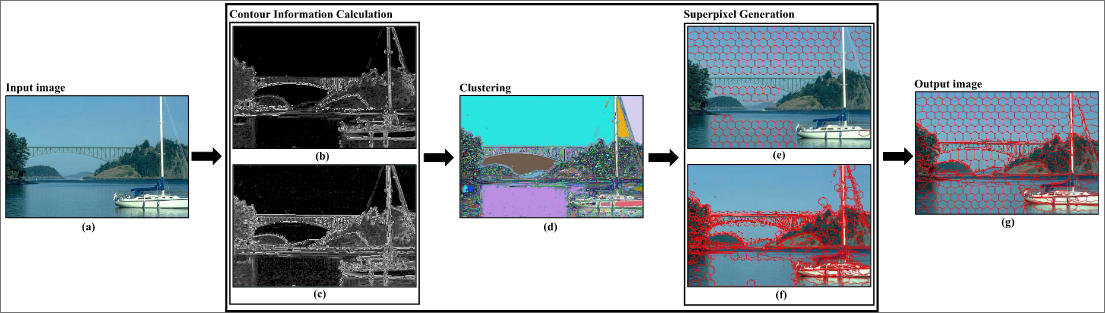
\includegraphics[width=1.0\textwidth]{pic/hqs.png}
	\caption{HQS超像素分割示意图}
      \label{fig:hqs_pic}
\end{figure}

\subsection{轮廓信息计算}
在图像处理领域,轮廓信息计算是一个重要的步骤,它帮助算法更好地区分图像中的像素,尤其是在颜色相似但属于不同语义区域的像素之间。为了获得轮廓信息,首先对图像进行边缘检测,得到边缘图,并通过非最大值抑制处理来细化边缘,使其成为单个像素宽的线段。在这一过程中,可能会丢失一些边界点,因此需要通过设定边界点的局部区域值来补充这些丢失的边界点,以确保轮廓信息的完整性。接下来,在CIELAB色彩空间的亮度通道上计算像素的轮廓信息,这通常涉及到计算像素的梯度值,这些值反映了像素在不同方向上灰度值的变化。通过设定阈值,可以判断像素是否位于图像的平坦区域,相应地生成4邻域和8邻域的轮廓信息。

公式 \eqref{eq:around4} 为对于像素 \(p\) 的4邻域梯度值计算公式。其中,\(t_h\)​ 和 \(t_v​\)​ 分别代表像素 \(p\) 在水平和垂直方向上的灰度变化。

\begin{equation}
  \hat{t} = \sqrt{(t_h)^2 + (t_v)^2}
  \label{eq:around4}
\end{equation}

公式\eqref{eq:four}为4邻域轮廓信息 \(t\) 定义。这里 \(T\) 是一个阈值,用于区分平坦区域和非平坦区域。

\begin{equation}
  t = \begin{cases}
    0, & \hat{t} < T \\
    \hat{t}, & \text{otherwise}
  \end{cases}
  \label{eq:four}
\end{equation}

这些轮廓信息随后被用于聚类过程,与颜色和空间信息结合起来,以增强算法对像素之间细微差别的识别能力,特别是在图像的边缘附近。通过这种轮廓信息的计算和应用,算法能够更精确地进行超像素的生成,从而在形状规则性和边界贴合度之间取得更好的平衡。

在HQS超像素分割算法中,轮廓信息的计算是通过使用RCF边缘检测算法来实现的。RCF算法是一种基于数学形态学的边缘检测方法,它通过在不同尺度上对图像进行处理来识别边缘。这种方法首先在多个尺度上对图像进行平滑和边缘响应的计算,然后通过一种竞争机制来选择最能够代表边缘的尺度,从而生成最终的边缘图。在HQS算法中,生成的边缘图随后会经过非最大值抑制处理,以细化边缘并减少由于噪声产生的假边缘。RCF边缘检测算法的核心在于利用卷积神经网络的强大特征提取能力来识别图像中的边缘。RCF算法首先对输入图像进行边缘检测,生成边缘图像,然后通过非极大值抑制处理来细化边缘,这一处理步骤移除边缘周围的非边缘像素,仅保留局部最大值点,从而形成更加精细和连续的边缘表示。

为了补充因非极大值抑制可能丢失的边界点,算法采用一种局部邻域平均值的方法来恢复边缘的完整性。随后,算法计算每个像素的轮廓信息,这涉及到评估像素梯度的大小,对于4邻域的像素,如果其梯度值小于预设阈值,则认为该像素位于图像的平坦区域,其轮廓信息被设置为0。HQS算法能够有效地提取图像中的重要轮廓信息,这些信息对于区分图像中颜色相似但属于不同区域的像素至关重要,有助于在后续的超像素生成步骤中生成形状更加规则且边界贴合度更高的超像素,从而为图像处理和计算机视觉任务提供高质量的超像素分割结果。\figref{fig:RCF}展示了RCF边缘检测结果图。

\begin{figure}[htbp]
	\centering
    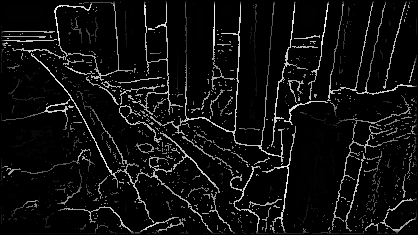
\includegraphics[width=0.5\textwidth]{pic/rcf/2.png}
	\caption{RCF边缘检测结果图}
      \label{fig:RCF}
\end{figure}

\newpage

\subsection{聚类}
在HQS超像素生成算法中,聚类步骤是通过精心设计的流程来实现的,这个流程首先涉及到对图像中每个像素的轮廓信息进行计算,这包括使用边缘检测技术来捕捉图像的边缘,并计算出像素的局部梯度,以此来增强对图像中平坦区域和非平坦区域的区分。接着,算法定义了一种新的邻域距离度量,它不仅考虑了像素之间的颜色差异,还结合了轮廓信息,从而更准确地衡量像素的相似性。基于这种度量,算法将视觉上相似的像素归纳到相似像素集中,并通过递归的方式将彼此认为是相似像素的像素分配到同一个类别中,实现了像素的聚类。\cite{achanta2012slic}公式 \eqref{eq:dist}为邻域距离 \( d(p, pm) \) 的计算公式。其中,\( l, a, b \) 和 \( l_m, a_m, b_m \) 分别是像素 \( p \) 和其邻居像素 \( pm \) 在CIELAB颜色空间中的值,\( t_m \) 是邻居像素 \( pm \) 的4邻域轮廓信息。

\begin{equation}
  d(p, pm) = t_m + \sqrt{(l - l_m)^2 + (a - a_m)^2 + (b - b_m)^2}
  \label{eq:dist}
\end{equation}

算法还特别区分了图像中的平坦区域和非平坦区域,以便采用不同的策略来处理这些区域,确保在平坦区域生成形状规则的超像素,在非平坦区域则生成边界贴合度更高的超像素。最后,算法在聚类的基础上生成种子点,这些种子点作为超像素的中心,被精心选择以反映出图像的区域特性,从而使得生成的超像素既规整又能够紧密贴合图像的真实边界。

\subsection{种子点生成}
在HQS超像素生成算法中,种子点的生成是一个精细的过程,它基于图像的聚类结果并考虑到像素的分布特性。算法首先在图像上构建一个规则的六边形网格,每个六边形都代表着一个潜在的超像素区域,其数量与期望生成的超像素数目相对应。在每个六边形内,算法通过一个限定的搜索区域内寻找种子点,这些种子点被选为超像素的中心,它们通常不会位于图像边缘,而是尽可能地靠近六边形的中心位置,以确保生成的超像素既大又对称。为了找到最佳的种子点,算法会计算候选像素到六边形中心的距离,并选择与周围像素类标签一致且距离中心最近的像素。公式\eqref{eq:seed}为种子点距离 \( ds(p, z) \) 的计算公式。其中,\( (x, y) \) 和 \( (x_z, y_z) \) 分别是像素 \( p \) 和六边形中心 \( z \) 的空间坐标。

\begin{equation}
  ds(p, z) = \sqrt{(x - x_z)^2 + (y - y_z)^2}
  \label{eq:seed}
\end{equation}

如果在六边形内找不到合适的种子点,算法会转而考虑颜色信息变化较小的区域,利用二阶差分梯度来衡量颜色复杂度,并选择复杂度最低的像素作为种子点。在超像素生成的迭代过程中,种子点会根据周围像素的特征进行更新,以维持超像素的一致性和形状规整性。通过这种方法,算法能够有效地生成既符合形状规则又紧密贴合图像真实边界的高质量超像素。

\subsection{超像素生成}
超像素生成是图像处理中的一项技术,旨在将图像分割成若干个较大的、视觉上相似且边界清晰的区域,这些区域被称为超像素。在HQS算法中,超像素的生成是一个分阶段的过程,它首先利用聚类结果和种子点来初始化超像素,然后在平坦区域和非平坦区域分别采用不同的策略来细化这些区域的超像素。
在平坦区域,图像的像素变化不大,因此可以快速地将这些区域的像素划分到较大的超像素中。而在非平坦区域,由于存在更多的纹理和轮廓变化,算法会采用自适应的参数和距离函数来更精确地生成超像素,以确保这些区域的超像素能够紧密贴合图像的真实边界。在生成过程中,算法还会不断地更新种子点的位置,并对超像素的形状进行调整,以提高超像素的规则性和视觉质量。为了进一步提升超像素的整体质量,算法还会执行一个合并步骤,将那些孤立的、细小的超像素与邻近的超像素合并,从而生成更加整洁和一致的超像素边界。整个过程通过迭代的方式进行,直到达到预定的超像素数量或者满足其他终止条件。最终,超像素生成算法能够产生一组既规整又具有强边界贴合度的超像素,这些超像素可以作为许多计算机视觉任务的有效预处理步骤。\figref{fig:hqs}展示了HQS超像素分割的结果。

\begin{figure}[htbp]
	\centering
    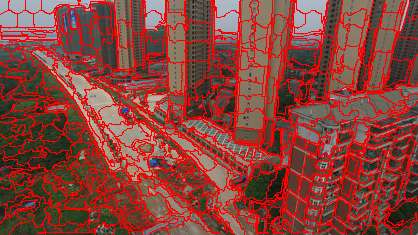
\includegraphics[width=0.5\textwidth]{pic/hqs/500/2.png}
	\caption{HQS超像素分割结果图}
      \label{fig:hqs}
\end{figure}

\newpage

\section{实验设计及算法评估}
在HQS超像素生成算法的实验设计和评估中,本文采用了标准的公开数据集,如UAVid数据集,这些数据集包含了丰富的无人机图像内容,并配有人工标注的地面真实(Ground Truth)分割,为算法提供了有力的评估基准。为了全面评估算法的性能,本文选择了精确率(Acc)、召回率(Recall)、平均交并比(MIoU)、卡帕指数(Kappa)这四个常用的超像素评估指标。这些指标不仅考虑了超像素的形状规则性和边界贴合度,还衡量了超像素内部的颜色一致性和与真实图像边界的对齐程度。在实验中,本文将HQS算法与其他多种现有的先进超像素生成方法进行了比较,包括SLIC、LSC、SEEDS。本文不仅对算法的数值结果进行了比较,还进行了可视化的比较,展示了不同算法生成的超像素在图像中的分布和外观。本文还探讨了HQS算法在实际无人机视觉任务中的应用,例如使用超像素作为显著性检测任务的预处理步骤,进一步证明了HQS算法在实际应用中的有效性和优势。通过这些综合的实验设计和评估,本文展示了HQS超像素生成算法在无人机领域的先进性能和应用潜力。

\subsection{实验环境}
\subsubsection{实验环境介绍}

本次实验的实验环境为Intel(R) Core(TM) i7-10510U CPU @ 1.80GHz处理器、16GB运行内存、Ubuntu 22.04操作系统、Python 3.11、gcc(GCC)13.2.1、Opencv4.9.0、cuda 12.4.r12.4。以下为实验环境的具体介绍:

\begin{enumerate}
\item Intel(R) Core(TM) i7-10510U CPU @ 1.80GHz 是一款由Intel公司生产的中央处理器,属于其第10代Core系列。i7是Intel的高端处理器系列之一,通常提供较强的性能。这款处理器的基础时钟频率为1.80吉赫兹(GHz),意味着它的处理核心每秒可以执行18亿次周期性操作。

\item 16GB运行内存(RAM)表示系统拥有16吉字节(GB)的随机存取存储器。对于大多数现代计算机应用来说,这是一个相对充足的内存容量,可以支持多任务处理和内存密集型应用。

\item Ubuntu 22.04 操作系统是一款基于Linux的开源操作系统,由Canonical Ltd公司开发。Ubuntu以其用户友好的图形用户界面和强大的命令行工具而闻名,广泛用于个人电脑、服务器和云计算环境。

\item Python 是一种广泛使用的高级编程语言,以其简洁的语法和强大的标准库而受到青睐。它支持多种编程范式,包括面向对象、命令式、函数式和过程式编程。Python 3.11是该语言的最新主要版本,包含了许多新特性和性能改进。

\item GCC 是 GNU Compiler Collection(GNU 编译器套件)的一个较新版本,它是一套广泛使用的编译器,支持多种编程语言。

\item Opencv 全称是Open Source Computer Vision Library,即开源计算机视觉库,是一个功能强大的计算机视觉和机器学习库。自从2000年由Intel的程序员创立以来,OpenCV已经成为计算机视觉领域最流行的工具之一。其中opencv contrib是OpenCV的额外贡献模块,包含了一些额外的算法和功能。

\item CUDA(Compute Unified Device Architecture)是由NVIDIA开发的一种并行计算平台和编程模型,它允许软件开发者和软件工程师使用NVIDIA GPU进行高性能计算(HPC)的开发。

\end{enumerate}

\subsubsection{实验环境搭建}

为了进行本文的研究,在Ubuntu系统上搭建实验环境,尤其是涉及cuda、cudann、OpenCV及其附加模块opencv contrib,可以遵循以下大致流程:

\begin{enumerate}
\item 更新Ubuntu系统到最新版本。
\item 下载适合的GPU架构和操作系统的CUDA Toolkit版本。下载完成后,解压缩安装包,并根据提供的文档指示,设置环境变量,以及将CUDA的二进制文件路径添加到PATH。下载与CUDA Toolkit兼容的cuDNN版本,解压后将库文件、包含文件和可执行文件复制到CUDA Toolkit的相应目录下。使用CUDA Toolkit提供的sample来验证安装是否成功。
\item 安装编译OpenCV所需的基本工具和库,如 build-essential、cmake、git、libgtk2.0-dev、pkg-config、libavcodec-dev、libavformat-dev、libswscale-dev 等。
\item 获取OpenCV和opencv contrib源码。
\item 使用CMake配置编译选项,确保包含opencv contrib。
\item 使用make编译Opencv源码。
\item 编译完成后,将OpenCV安装到系统中。
\end{enumerate}

\subsection{实验准备}
\subsubsection{数据集准备}

UAVid数据集是一个为无人机(UAV)影像设计的高分辨率语义分割数据集,它主要针对城市场景的语义分割任务。该数据集包含从30个视频序列中捕获的300张高分辨率图像,这些图像被标记为8个不同的对象类别。UAVid数据集的特点是它提供了倾斜视角下的无人机图像,这使得数据集能够捕捉到物体的顶视图和侧视图,为对象识别提供了更多的信息。UAVid数据集面临的挑战包括处理不同距离或不同类别物体之间的大规模变化、城市街道场景中的移动物体识别,以及保持时间一致性以更好地进行跨帧预测。这些挑战使得UAVid数据集在语义分割任务中具有独特性。UAVid数据集包含的图像分辨率高,这为精确的语义分割提供了更丰富的细节,但同时也增加了处理的复杂性。数据集中的图像是从倾斜视角捕获的,这意味着它们不仅包含物体的顶视图,还包含侧视图,这为对象识别提供了更全面的视角。UAVid数据集包含8个不同的对象类别,这要求分割模型能够识别并区分多种不同的城市地物目标。数据集中的图像需要处理不同距离和不同类别物体之间的大规模变化,这对模型的泛化能力提出了更高的要求。城市街道场景中包含移动物体,如车辆和行人,这增加了分割任务的难度,因为模型需要能够识别并跟踪这些物体。为了更好地进行跨帧预测,UAVid数据集需要保持时间一致性,这意味着模型不仅要在单帧内进行准确的分割,还要能够在连续的视频帧之间保持一致的识别结果。

UAVid数据集的规模是一些现有数据集的数倍,如Vaihingen、CamVid和波茨坦数据集,这为研究提供了更丰富的数据,但同时也带来了更大的计算挑战。由于无人机影像的实时性和动态性,UAVid数据集中的某些目标可能在数据采集前无法事先确定,这要求分割模型具有较高的适应性和鲁棒性。UAVid数据集的这些特点和挑战使得它在语义分割领域具有重要价值,同时也推动了相关算法的发展和创新。\tabref{tab:uavid}展示了部分数据集。

\begin{table}[htbp]
    \centering
    \caption{部分无人机图像}
      \begin{tabular}{ccccc}
        \toprule
        filename & picture  & filename  & picture \\
        \midrule
        2.png & 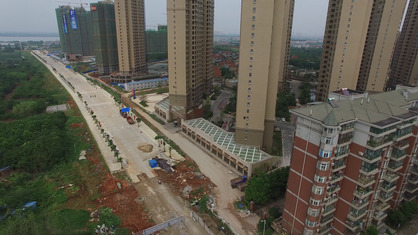
\includegraphics[width=0.2\textwidth]{pic/raw/2.png} & 71.png & 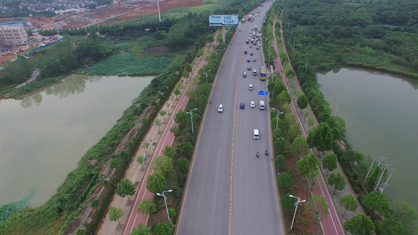
\includegraphics[width=0.2\textwidth]{pic/raw/71.png} \\
        42.png & 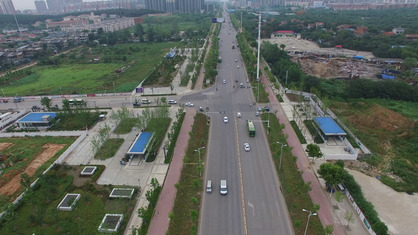
\includegraphics[width=0.2\textwidth]{pic/raw/42.png} & 82.png & 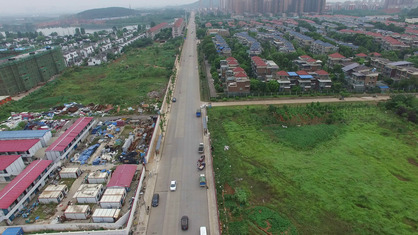
\includegraphics[width=0.2\textwidth]{pic/raw/82.png} \\
        44.png & 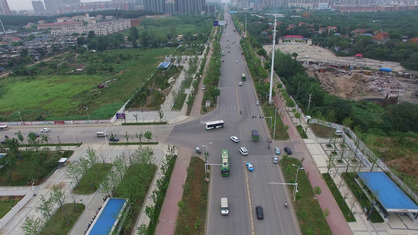
\includegraphics[width=0.2\textwidth]{pic/raw/44.png} & 83.png & 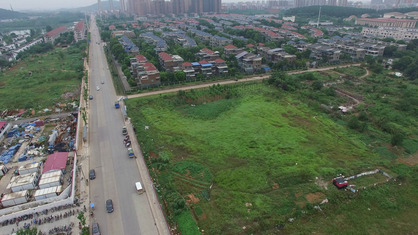
\includegraphics[width=0.2\textwidth]{pic/raw/83.png} \\
        47.png & 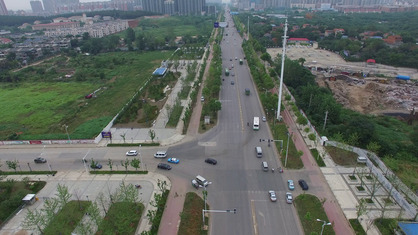
\includegraphics[width=0.2\textwidth]{pic/raw/47.png} & 90.png & 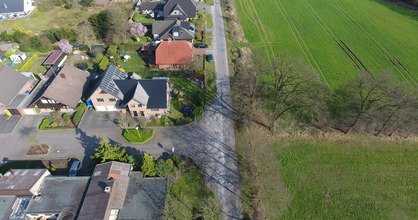
\includegraphics[width=0.2\textwidth]{pic/raw/90.png} \\
        48.png & 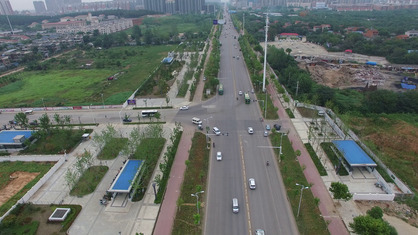
\includegraphics[width=0.2\textwidth]{pic/raw/48.png} & 130.png & 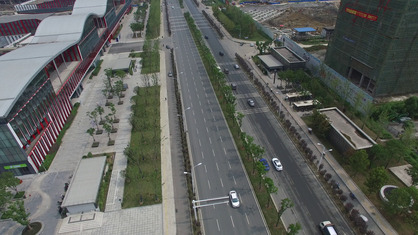
\includegraphics[width=0.2\textwidth]{pic/raw/130.png} \\
        50.png & 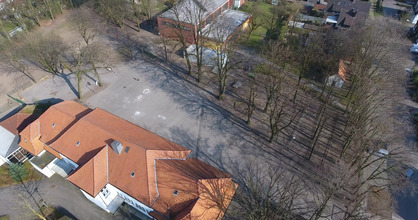
\includegraphics[width=0.2\textwidth]{pic/raw/50.png} & 131.png & 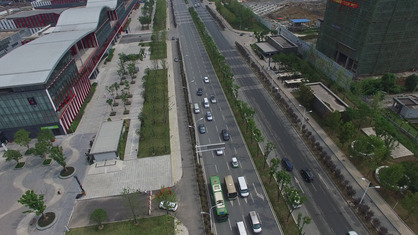
\includegraphics[width=0.2\textwidth]{pic/raw/131.png} \\
        55.png & 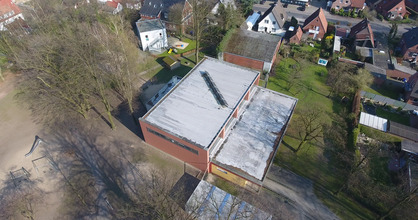
\includegraphics[width=0.2\textwidth]{pic/raw/55.png} & 135.png & 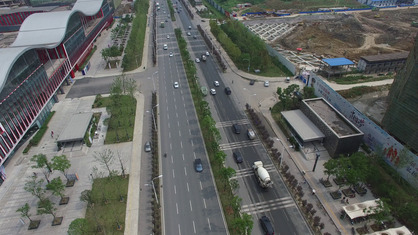
\includegraphics[width=0.2\textwidth]{pic/raw/135.png} \\
        60.png & 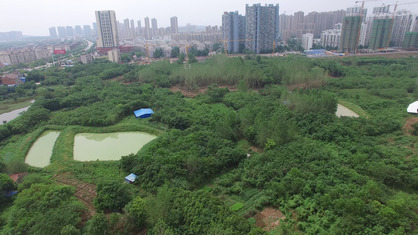
\includegraphics[width=0.2\textwidth]{pic/raw/60.png} & 139.png & 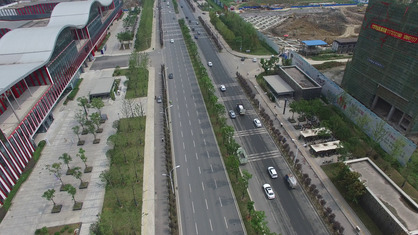
\includegraphics[width=0.2\textwidth]{pic/raw/139.png} \\
        \bottomrule
    \end{tabular}%
    \label{tab:uavid}%
  \end{table}%

  \newpage

为了测试数据集的可用性,UAVid提供了几种典型的深度神经网络基线方法,包括FCN-8s、Dilation Net和U-Net,这些网络在不同数据集的语义分割任务中被广泛使用和验证。UAVid还提出了一种新颖的多尺度扩张网络,用于处理数据集中突出的大规模变化问题,并应用了现有的时空正则化方法,如特征空间优化(FSO)和3D条件随机场(CRF),以保持跨帧的一致预测。在UAVid数据集的基础上,使用Canny边缘检测提取无人机图像轮廓,然后通过非极大值抑制和条件随机场(CRF)进一步精细化边缘,为图像分割算法提供高质量的输入。Canny算法能够突出图像中的边缘信息,而非极大值抑制则有助于去除边缘中的噪声,确保边缘的连贯性。CRF作为一种强大的后处理工具,能够利用像素之间的空间关系,对边缘进行平滑处理,提高分割的准确性。

结合这些技术,可以显著提升分割算法在处理UAVid数据集时的性能,尤其是在面对大规模变化、移动物体识别以及保持时间一致性等挑战时。此外,多尺度特征提取和时空正则化的应用,使得模型能够更好地适应不同尺寸的物体,并且在视频序列中保持分割结果的一致性。UAVid数据集的这些特性和处理技术的结合,不仅推动了无人机影像语义分割技术的发展,而且为智能农业、精准农业、地籍测绘、杂草监测以及交通和人口密度监测等多个应用领域提供了强大的技术支持。


\subsubsection{对比模型}
为了全面验证创新模型HQS超像素分割的性能,本文中将引入另外三个超像素分割的经典算法作为对比。以下是对三种算法的介绍:

1. SLIC超像素分割算法是一种流行的基于网格的聚类方法,它通过将图像分割成小块的超像素,然后根据这些像素之间的颜色和空间邻近性进行合并,从而生成视觉上更加紧凑和均匀的区域。这种方法因其在图像分割任务中的有效性而受到青睐,能够产生形状规则且大小一致的超像素,这对于后续的图像处理任务如目标检测、图像分割和图像分类等非常有用。

2. SEEDS算法作为一种层次聚类算法,其核心思想是从每个单独的数据点开始,将每个点视为一个初始的簇,然后根据定义的相似度指标逐步合并这些簇。这种方法的优势在于它能够自然而然地适应簇的不同形状和大小,而不是强制将数据划分为预先指定数量的簇,这使得SEEDS算法在处理复杂数据结构时更加灵活和有效。但是,SEEDS算法也有其局限性。由于层次聚类需要在所有数据点之间计算相似度并进行多次合并操作,这可能导致计算开销较大,尤其是在处理大规模数据集时更为明显。层次聚类算法通常对噪声和异常值比较敏感,这些因素可能会影响簇的合并过程,从而改变最终的聚类结果。

3. LSC算法,即线性谱聚类算法,是一种基于图论的聚类方法,它在图像分割和数据分析中得到了广泛应用。LSC算法的工作原理是首先构建一个图,其中的数据点作为图的节点,节点之间的连接关系(边)基于数据点的局部邻域信息来确定。算法利用谱分析技术来处理这个图,通过分析图的拉普拉斯矩阵的特征向量来发现数据点之间的固有联系,并据此形成簇。LSC算法的一个显著优点是其能够识别和捕捉数据中复杂的簇结构,即使在簇形状不规则或存在重叠时也能有效地进行聚类。由于谱分析的特性,LSC算法对噪声和异常值具有较强的鲁棒性,这使得它在处理现实世界中常见的不完美数据时更为可靠。与需要预先指定簇数量的算法相比,LSC算法不需要这样的先验知识,从而简化了聚类过程。

通过将HQS算法与SLIC、SEEDS、LSC等其他聚类算法进行对比,可以全面地验证HQS在无人机图像分割任务中的性能。这种对比不仅有助于确定HQS在准确性、效率和鲁棒性方面的表现,而且还可以作为评估其在特定应用场景,如无人机图像分析中的适应性和实用性的基准。观察HQS在参数调整方面的敏感性,可以指导如何在不同场景下优化算法性能。通过引入噪声和异常值的测试可以展现HQS的健壮性,尤其是在对噪声敏感的算法对比中。计算效率的对比可以突出HQS在处理大规模数据集时的优势,尤其是在需要实时或近实时分割处理的应用中。

\subsubsection{实验过程}
本文实现了HQS超像素分割算法,比较HQS超像素分割与SLIC,LSC,SEEDS 这三个基准模型在各个方面的差距,以验证HQS超像素分割是否适用于无人机图像。且一共四个个模型将在 UAVid 数据集全部进行测试,以帮助本文全面地评估模型的性能,包括其可扩展性、性能边界、稳健性以及在真实世界应用中的表现。

实验的第一步是使用Canny算法对图像进行边缘检测预处理,这一步骤有助于增强图像的边缘信息,为后续的轮廓信息提取提供坚实的基础。本文应用了NSM(Non-Maximum Suppression)和RCF算法,这些算法旨在进一步提炼图像的纹理和轮廓特征,从而为HQS算法提供了更加精确的输入。在图像经过这些预处理步骤之后本文引入了HQS算法。HQS算法通过其独特的区域分解技术,将图像划分为平坦和非平坦区域,并根据这些区域的特点采取相应的分割策略。对于平坦区域,HQS算法可能会采用更宽松的聚类标准来保持区域的连贯性;而在非平坦区域,算法则可能采用更严格的标准来捕捉更多的细节。这一过程中,轮廓信息的计算非常关键,它确保了超像素的边界尽可能地与图像中的真实轮廓对齐。HQS算法通过其独特的区域分解技术,将图像划分为平坦和非平坦区域,并针对这些不同区域采取了相应的分割策略,以生成既规则又贴合图像真实边界的超像素。这一分割过程涉及到轮廓信息的计算、像素聚类、种子点的生成和超像素的生成与合并等关键步骤。

最终,本文对HQS算法生成的超像素进行了详尽的分析。这包括了对超像素质量的定量评估,如边界贴合度、形状规则性、以及与基准模型的比较等。本文还考虑了算法的计算效率,以及在不同图像内容和条件下的适应性和稳健性。实验结果的分析不仅涉及了数值统计,还包括了可视化展示,这些都是为了更全面地理解HQS算法在无人机图像分割任务中的表现。

\subsection{对比实验结果以及分析}

\subsubsection{实验结果}

\tabref{tab:result}展示了实验结果图。第一列为原图的文件名,第二列为原图,第三列为RCF边缘检测的结果图像,第四列为HQS图像分割结果,第五列为Ground Truth。

\begin{table}[htbp]
    \centering
    \caption{实验结果}
    \begin{tabular}{ccccc}
      \toprule
      filename & raw & RCF & HQS superpixels & ground truth \\
      \midrule
      2.png & 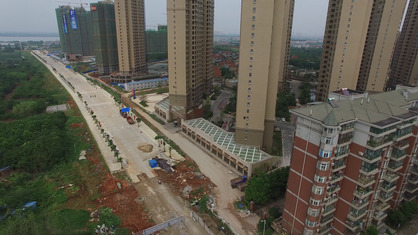
\includegraphics[width=0.2\textwidth]{pic/raw/2.png} & 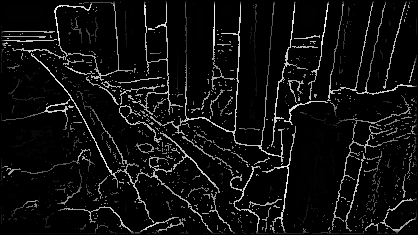
\includegraphics[width=0.2\textwidth]{pic/rcf/2.png} & 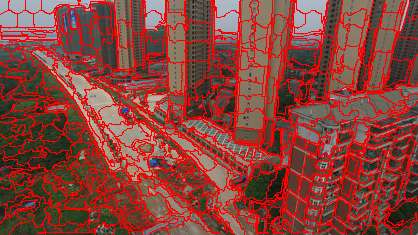
\includegraphics[width=0.2\textwidth]{pic/hqs/500/2.png} & 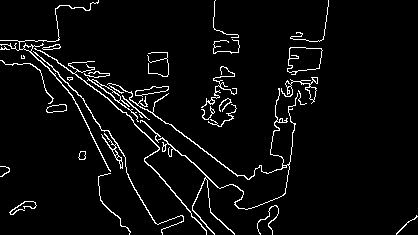
\includegraphics[width=0.2\textwidth]{pic/gt/2.png} \\
      42.png & 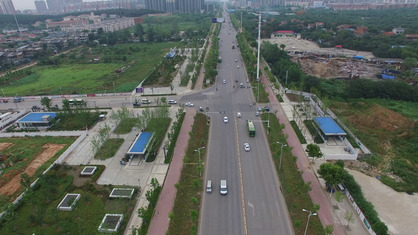
\includegraphics[width=0.2\textwidth]{pic/raw/42.png} & 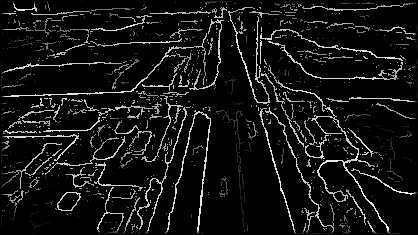
\includegraphics[width=0.2\textwidth]{pic/rcf/42.png} & 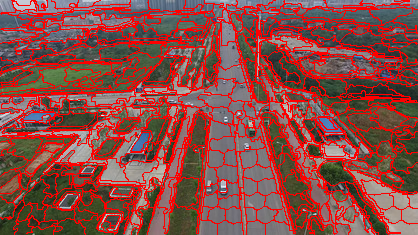
\includegraphics[width=0.2\textwidth]{pic/hqs/500/42.png} & 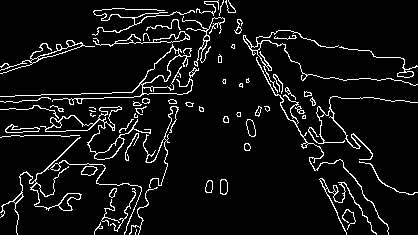
\includegraphics[width=0.2\textwidth]{pic/gt/42.png} \\
      47.png & 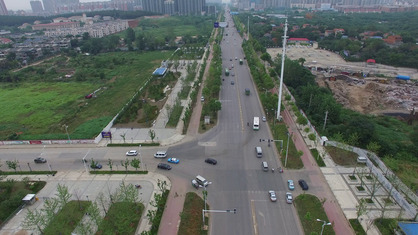
\includegraphics[width=0.2\textwidth]{pic/raw/47.png} & 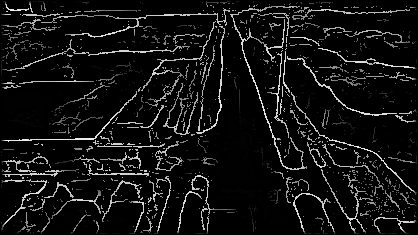
\includegraphics[width=0.2\textwidth]{pic/rcf/47.png} & 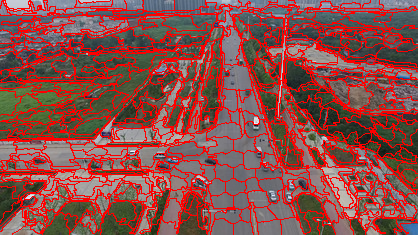
\includegraphics[width=0.2\textwidth]{pic/hqs/500/47.png} & 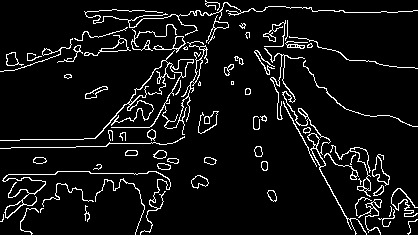
\includegraphics[width=0.2\textwidth]{pic/gt/47.png} \\
      48.png & 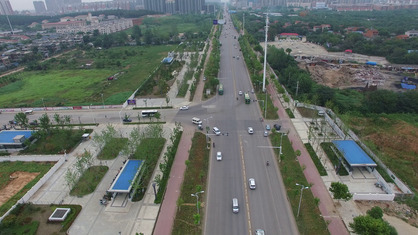
\includegraphics[width=0.2\textwidth]{pic/raw/48.png} & 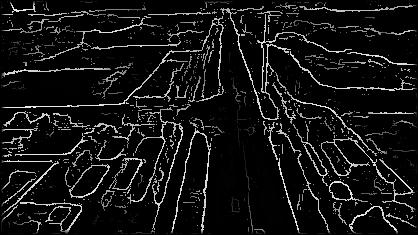
\includegraphics[width=0.2\textwidth]{pic/rcf/48.png} & 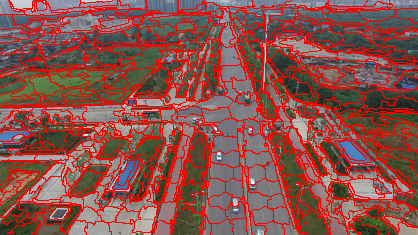
\includegraphics[width=0.2\textwidth]{pic/hqs/500/48.png} & 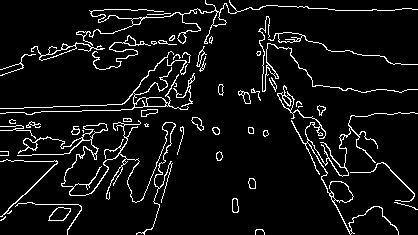
\includegraphics[width=0.2\textwidth]{pic/gt/48.png} \\
      50.png & 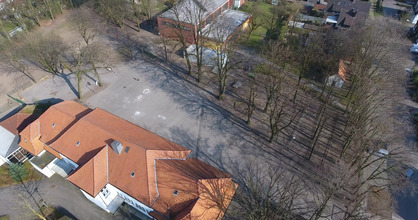
\includegraphics[width=0.2\textwidth]{pic/raw/50.png} & 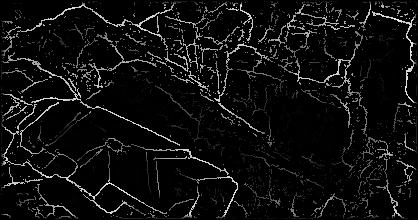
\includegraphics[width=0.2\textwidth]{pic/rcf/50.png} & 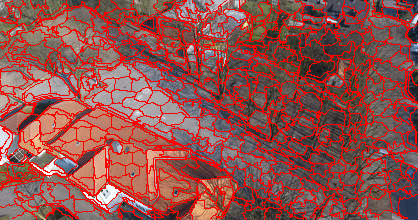
\includegraphics[width=0.2\textwidth]{pic/hqs/500/50.png} & 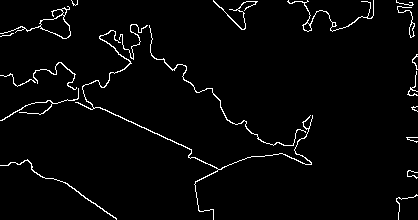
\includegraphics[width=0.2\textwidth]{pic/gt/50.png} \\
      55.png & 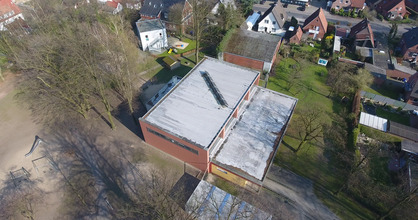
\includegraphics[width=0.2\textwidth]{pic/raw/55.png} & 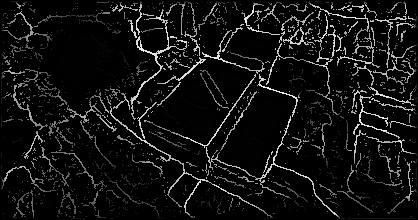
\includegraphics[width=0.2\textwidth]{pic/rcf/55.png} & 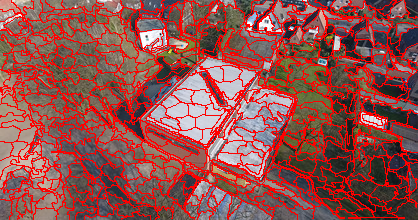
\includegraphics[width=0.2\textwidth]{pic/hqs/500/55.png} & 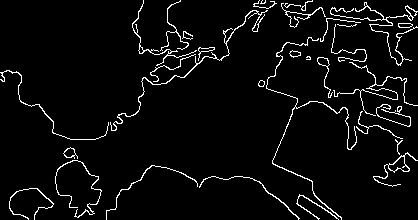
\includegraphics[width=0.2\textwidth]{pic/gt/55.png} \\
      60.png & 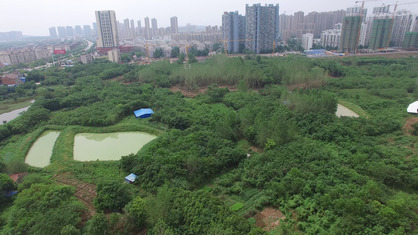
\includegraphics[width=0.2\textwidth]{pic/raw/60.png} & 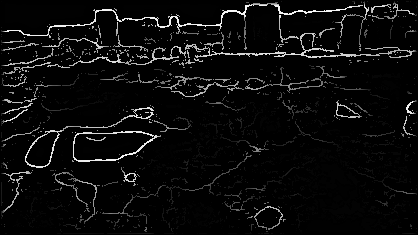
\includegraphics[width=0.2\textwidth]{pic/rcf/60.png} & 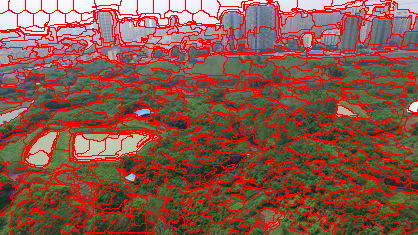
\includegraphics[width=0.2\textwidth]{pic/hqs/500/60.png} & 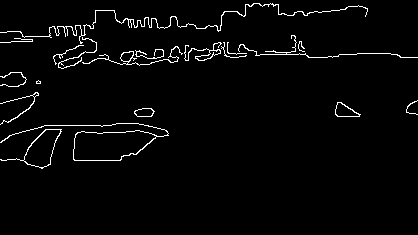
\includegraphics[width=0.2\textwidth]{pic/gt/60.png} \\
      71.png & 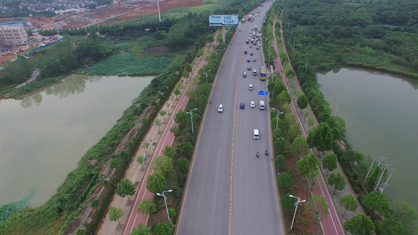
\includegraphics[width=0.2\textwidth]{pic/raw/71.png} & 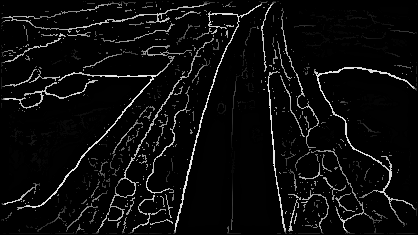
\includegraphics[width=0.2\textwidth]{pic/rcf/71.png} & 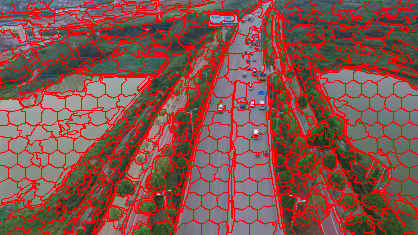
\includegraphics[width=0.2\textwidth]{pic/hqs/500/71.png} & \includegraphics[width=0.2\textwidth]{pic/gt/71.png} \\
      82.png & \includegraphics[width=0.2\textwidth]{pic/raw/82.png} & \includegraphics[width=0.2\textwidth]{pic/rcf/82.png} & \includegraphics[width=0.2\textwidth]{pic/hqs/500/82.png} & \includegraphics[width=0.2\textwidth]{pic/gt/82.png} \\
      \bottomrule
    \end{tabular}
    \label{tab:result}
  \end{table}

  \newpage

\subsubsection{实验结果可视化}
在进行超像素分割的过程中,记录每个图下六种方法的召回率 (Recall)、准确率 (Acc)、帕系数 (Kappa)、F1系数(F1)、交并比(IoU)、平均交并比 (MIoU)。最显眼的橙色为本文的HQS超像素分割。

\begin{figure}[htbp]
	\centering
	\includegraphics[width=1\textwidth]{pic/Recall.png}
	\caption{Recall指标对比图}
    \label{fig:recall}
\end{figure}

如\figref{fig:recall}所示,HQS算法的召回率最高。这表明在使用HQS算法进行超像素分割时,模型能够较好地识别出大部分应该被识别的区域,具有较高的敏感性。SLIC算法的召回率也相对较高,但低于HQS算法。而LSC算法和SEEDS算法的召回率则稍低,这可能意味着在某些情况下,LSC算法和SEEDS可能会遗漏更多的实际分割区域。图像中不同图像文件对应的召回率有所波动,这可能反映了不同图像的特点对算法性能的影响。例如,图像的复杂度、对比度和纹理等特征可能对超像素分割的性能有显著的影响。总体而言,HQS算法在召回率方面表现出色,而SLIC算法虽然表现良好,但在保持高召回率方面仍有提升空间。

\newpage

\begin{figure}[htbp]
	\centering
	\includegraphics[width=1\textwidth]{pic/Acc.png}
	\caption{Acc指标对比图}
    \label{fig:acc}
\end{figure}

如\figref{fig:acc}所示,从图像中可以看出,HQS算法表现最为出色,其准确性值接近0.85,这表明在这些测试图像上,HQS算法能够非常精确地识别和分割图像内容。另一方面,SLIC算法在某些图像上的准确性低于HQS,这意味着SLIC在这些情况下的准确性不如HQS算法。整体而言,这些结果揭示了HQS算法在这些测试条件下优越的准确性。

\begin{figure}[htbp]
	\centering
	\includegraphics[width=1\textwidth]{pic/Kappa.png}
	\caption{Kappa指标对比图}
    \label{fig:kappa}
\end{figure}

如\figref{fig:kappa}所示,SEEDS算法的卡帕系数最高。这意味着SEEDS算法在这些图像的超像素分割任务中实现了相对较高的一致性。HQS算法的卡帕系数较低,这表明HQS算法在保持分类一致性方面的表现不如前两者。此外,不同图像的卡帕系数存在波动,这可能反映了图像内容的多样性对超像素分割算法性能的影响。例如,图像中的内容、纹理、对比度和结构的复杂性都可能对分割算法的一致性造成挑战。总体而言,HQS算法在卡帕系数方面不如SEEDS、LSC、SLIC。SEEDS算法在这些测试图像上展现出了较好的一致性表现。

\begin{figure}[htbp]
	\centering
	\includegraphics[width=1\textwidth]{pic/F1.png}
	\caption{F1指标对比图}
    \label{fig:F1}
\end{figure}

如\figref{fig:F1}所示,SEEDS方法在F1分数上表现最为出色,这表明SEEDS在处理相关任务时,能够很好地平衡精确度和召回率,实现较高的准确识别率。紧随其后的是HQS方法,虽然略低于SEEDS,但依然显示了很强的性能,说明HQS在大多数情况下能够可靠地识别目标。LSC方法的F1分数依然很高,表明LSC方法在任务中的表现也是相当可靠的,尽管略逊于前两名。SEEDS和HQS在F1分数上的表现较为突出,而SLIC可能需要进一步的优化来提升其性能。

\newpage

\begin{figure}[htbp]
	\centering
	\includegraphics[width=1\textwidth]{pic/IoU.png}
	\caption{IoU指标对比图}
    \label{fig:iou}
\end{figure}

如\figref{fig:iou}所示,SEEDS算法显示出在图像分割任务中较高的准确度和效率。紧随其后的是HQS方法,表明其性能与SEEDS相差无几,同样能够取得较好的分割效果。LSC虽然略低于前两者,但依然保持了较高的准确度。然而,SLIC方法在某些情况下不如前述方法稳定。

\begin{figure}[htbp]
	\centering
	\includegraphics[width=1\textwidth]{pic/MIoU.png}
	\caption{MIoU指标对比图}
    \label{fig:miou}
\end{figure}

如\figref{fig:miou}所示,HQS算法的平均交并比最高,这意味着HQS算法在这些图像的超像素分割任务中,预测的超像素与真实分割区域之间的重叠度较高,因此分割效果较好。紧随其后的是SLIC算法,LSC与SEED算法表现相当。结果表明SLIC其分割的准确性略低于HQS算法。LSC算法和SEEDS算法其MIoU值最低,这表明其在无人机分割任务中的表现需要进一步改进。总体而言,HQS算法和SLIC算法在这些测试图像上表现出了较好的分割性能,而LSC算法和SEEDS算法则在平均交并比这一指标上有所欠缺。

\subsubsection{实验结果分析}

在对HQS、SLIC、LSC和SEEDS四种超像素分割算法的性能评估中,我们可以观察到它们在不同指标上各有优势。HQS算法在召回率和准确性方面表现最为出色,这意味着它能够有效地识别出图像中应该被分割的区域,并且能够非常精确地进行分割。然而,尽管HQS算法在识别能力上很强,但在保持分类一致性方面,SEEDS算法则表现得更为优秀,显示出较高的卡帕系数,表明其分割结果与真实分割区域之间的一致性更好。
SLIC算法在召回率和MIoU上也展现了良好的性能,尽管在准确性上略逊于HQS算法,但其分割的准确性和预测超像素与真实分割区域之间的重叠度仍然值得肯定。相比之下,LSC算法和SEEDS算法在这些测试图像上的表现则显得有些不足,特别是在MIoU这一指标上,它们的值较低,暗示着在无人机分割任务中可能需要进一步的优化和改进。总体而言,HQS算法在多个关键指标上都显示出了较强的性能,而SLIC算法也是一个有力的竞争者。与此同时,SEEDS算法在一致性方面的优势不容忽视,而LSC和SEEDS算法则可能需要针对特定类型的图像或应用场景进行调整,以提升其分割性能。

综上所述,HQS算法在多个评价指标上都展现出了优秀的性能,较其他方法具有更好的边缘一致性和更规则的超像素分割边界。而SLIC算法在分割精度上也表现不俗。SLIC算法虽然在某些方面表现良好,但在精确度和召回率的平衡上还有改进的空间。LSC算法则需要在分割精度上进行进一步的优化。
